\section{梯度下降法}梯度下降法(Gradient Descent, GD)是求解无约束优化问题的一种最常见的方法\cite{6302929},在最优化、统计学以及机器学习等领域都有着广泛的应用,例如用梯度下降法求解最小二乘问题\cite{1989Least},在本章的末尾会有相应例题。对于无约束最优化问题:
\begin{equation}
    \min _{x}\left\{f(\bm{x}) \mid \bm{x} \in \mathbb{R}^{n}\right\} ,
    \label{eqt5_1}
\end{equation}
其中目标函数$f: \mathbb{R}^{n} \rightarrow \mathbb{R}$是连续可微$L$-光滑的函数。最优化问题\ref{eqt5_1}可以看作为一般问题\ref{eqt1_11}不加约束的特殊情况。由推论\ref{the1_4}可知,凸优化问题的最优解等价于梯度为零的解,即 $\bm{x}$ 满足$\nabla f(\bm{x})=0$。如果$\nabla f(\bm{x}) \neq 0$,那么根据函数$\bm{f(\bm{x})}$在$\bm{x}$处泰勒展开的性质可知,一定存在$\delta$,使得
\begin{equation}
    f(\bm{x}-\alpha \nabla f(\bm{x}))<f(\bm{x}), \quad \forall \alpha \in(0, \delta) .
    \label{eqt5_2}
\end{equation}
式\ref{eqt5_2}也表示$\bm{x}$梯度的反方向,即$-\nabla f(\bm{x})$,是目标函数值的下降方向。进一步,可以将这一下降现象推广到更一般的情形。如果方向$\bm{d} \in \mathbb{R}^{n}$满足
\begin{equation}
    \nabla f(\bm{x})^{\top} \bm{d}<0 ,
    \nonumber
\end{equation}
即方向 $d$ 与梯度方向$\nabla f(\bm{x})$的夹角大于90°,此时一定存在$\sigma$,满足:
\begin{equation}
    f(\bm{x}+\alpha \bm{d})<f(\bm{x}), \quad \forall \alpha \in(0, \delta) .
    \label{eqt5_3}
\end{equation}
沿着满足该性质的方向$\bm{d}$更新$\bm{x}$可以使目标函数下降,从而达到减小函数值的目的。
\begin{figure}[hbtp]
    \centering
    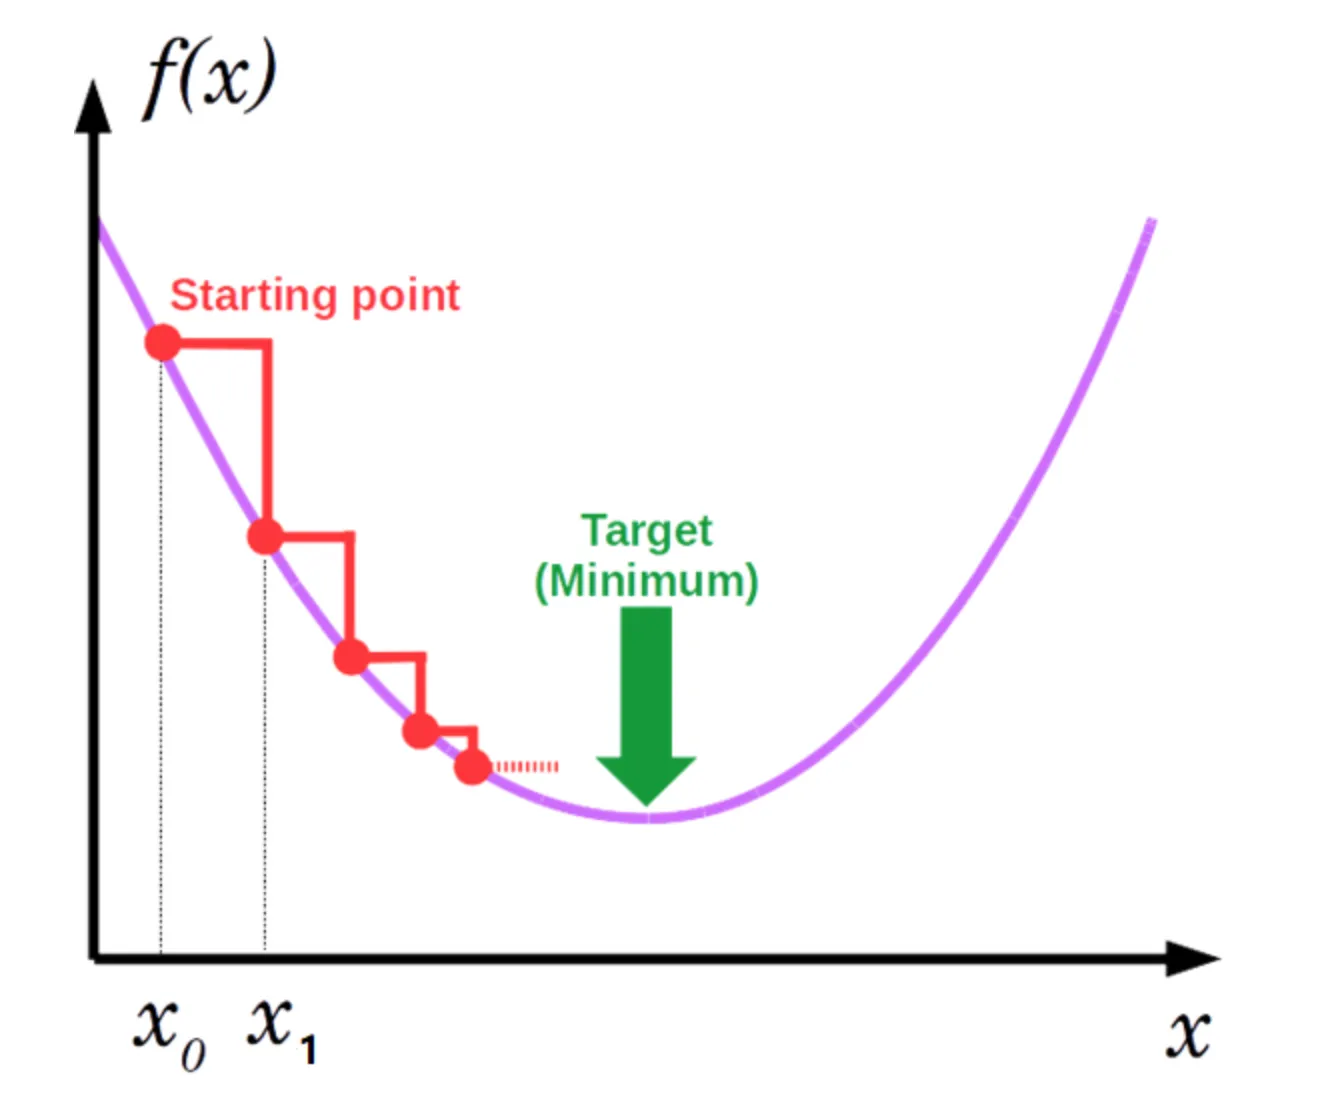
\includegraphics[width=100mm]{./Figures/gd-emp.png}
    \caption{寻找$\min f(\bm{x})$的过程}
    \label{figure_gd_emp}
\end{figure}

\subsection{梯度下降法}
一种凸优化模型通常通过人工设计迭代格式的方式来构建优化变量迭代序列$\left\{\bm{x}^{k}\right\}$,从而寻找问题的最优解,理论上需要建立所得到的迭代序列收敛到最优解的证明\cite{6302929}。梯度下降法,作为最简单常用的梯度类方法,是典型的以迭代格式进行最优化问题求解的算法,其具体的第$k+1$步的迭代格式如下:
\begin{equation}
    \bm{x}^{k+1}=\bm{x}^{k}-\alpha_{k} \nabla f\left(\bm{x}^{k}\right),
    \label{eqt5_4}
\end{equation}
其中$k$对应于迭代步数,$\alpha_{k}>0$称为步长 (step-size)或学习率 (learning rate)。梯度下降法的迭代格式\ref{eqt5_4}也可以从最优性条件的角度来理解,无约束优化问题\ref{eqt5_1}的最优性条件等价于
\begin{equation}
    \nabla f\left(\bm{x}^{*}\right)=0 \quad \Leftrightarrow \quad \bm{x}^{*}=\bm{x}^{*}-\alpha \nabla f\left(\bm{x}^{*}\right) ,
    \nonumber
\end{equation}
以不动点迭代的形式可以将该等价条件改写为梯度下降算法的迭代格式。如果所得到的序列$\left\{\bm{x}^{k}\right\}$是收敛的且收敛到$\bm{x}^{*}$,步长$\alpha_{k}$也收敛到$\alpha_{\infty}$,那么对迭代格式\ref{eqt5_4}中取$k \rightarrow \infty$可以得到
\begin{equation}
    \bm{x}^{*}=\bm{x}^{*}-\alpha_{\infty} \nabla f\left(\bm{x}^{*}\right) .
    \nonumber
\end{equation}
该式子等价于$\nabla f\left(x^{*}\right)=0$,这也说明$x^{*}$满足一阶最优性条件,即成为最优化问题\ref{eqt5_1}的最优解。
\par 梯度下降法是针对无约束最优化问题求解的最基本算法,除了迭代格式外,步长$k$的设计方式影响问题的求解效率和能力。下面介绍一系列常用步长设计方式\cite{2009Accelerated}:
\\ (1) 常数步长准则:$\alpha_{k}=\ell$ ;
\\ (2) 极小化准则:$ \alpha_{k}=\arg \min _{\alpha \geq 0} f\left(\bm{x}^{k}-\alpha \nabla f\left(\bm{x}^{k}\right)\right), \alpha \in(0, \delta)$ ;
\\ (3) 逐步减少 (diminishing) 步长准则:步长  $\alpha_{k}$  满足
\begin{equation}
    \lim _{k \rightarrow \infty} \alpha_{k}=0, \quad \sum_{k=0}^{\infty} \alpha_{k}=\infty ;
    \nonumber
\end{equation}
\\ (4) Armijo\cite{1999Convergence}准则:$\delta \in\left(0, \frac{1}{2}\right)$,令 $\alpha$ 从初始值 $s$ 开始以 $\beta \in(0, 1)$ 的倍数逐步减小,即
\begin{equation}
    \left\{s, \beta s, \beta^{2} s, \cdots\right\} ,
    \nonumber
\end{equation}
直到 $\beta^{m} s$ 且首次满足
\begin{equation}
    f\left(x^{k}\right)-f\left(x^{k}-\alpha \nabla f\left(x^{k}\right)\right) \geq-\delta \alpha \nabla f\left(x^{k}\right)^{T} \nabla f\left(x^{k}\right) .
    \nonumber
\end{equation}
Armijo准则是一种常用的步长设计准则\cite{1999Convergence},其通过定量标准来协助选择合适步长,通过有限步最终可以找到满足条件的步长,常用于非凸优化问题的求解计算。

\subsection{梯度下降法收敛性分析}
对于最优化方法的收敛性理论分析,主要包括算法收敛性、算法局部收敛速度以及算法全局迭代复杂度等方面\cite{2002ConvergenceAnalysis}。算法收敛性(convergence)指的是算法得到的迭代序列$\left\{x^{k}\right\}$的序列收敛性,如是否有聚点、聚点是否满足最优性条件以及序列是否全局收敛等。算法局部收敛速度(convergence rate)指的是在已证明算法迭代序列收敛的前提下,算法迭代序列可以以某种可量化的速度收敛到最优解(可能是局部最优解),如线性收敛速度、超线性收敛速度、二次收敛速度等。收敛速度通常考虑的只是局部性质,即算法迭代到一定步数后序列所体现出来的性质。与此同时,另一种算法全局迭代复杂度(iteration complexity)刻画的是算法从初始点开始经过一定迭代步数后所能到达的“最优化”程度(距离最优解或最优函数值的程度),即经过 $k$ 步迭代后,算法得到的序列 $\left\{\bm{x}^{k}\right\}$ 满足性质:
\begin{equation}
    f\left(\bm{x}^{k}\right)-f\left(\bm{x}^{*}\right) \leq \varepsilon .
    \label{eqt5_5}
\end{equation}
\par 对于梯度下降法\ref{eqt5_4},在最优化问题\ref{eqt5_1}的目标函数 $f(\cdot)$ 是连续可微$L$-光滑的基础上,假设 $f(\cdot)$ 为凸函数。其中 $f(\cdot)$ 的$L$-光滑性质,意味着
\begin{equation}
    \|\nabla f(\bm{x})-\nabla f(\bm{y})\| \leq L\|\bm{x}-\bm{y}\|, \quad \forall \bm{x}, \bm{y} \in \mathbb{R}^{n} .
    \nonumber
\end{equation}

\begin{theorem}[收敛性]\label{thm1}
    对于无约束最优化问题\ref{eqt5_1}的目标函数 $f(\cdot)$ 是连续可微 $L$-光滑的凸函数,序列 $\left\{\bm{x}^{k}\right\}$ 为梯度下降法\ref{eqt5_4}得到的迭代序列,且步长 $\alpha_{k} \in\left(0, \frac{2}{L}\right)$ ,那么该序列 $\left\{\bm{x}^{k}\right\}$ 收敛到 $\bm{x}^{*}$ ,其中  $\bm{x}^{*}$ 是最优化问题\ref{eqt5_1}的全局最优解。梯度下降法的迭代复杂度为
    \begin{equation}
        f\left(\bm{x}^{k}\right)-f\left(\bm{x}^{*}\right) \leq \mathcal{O}\left(\frac{1}{k}\right) .
        \nonumber
    \end{equation}
\end{theorem}

\begin{proof}
    首先,根据函数 $f(\cdot)$ 的$L$-光滑性质以及下降引理\ref{thm435},对于任意的 $\bm{x}, \bm{y} \in   \mathcal{D}$ 有
    \begin{equation}
        f(\bm{y}) \leq f(\bm{x})+\langle\nabla f(\bm{x}), \bm{y}-\bm{x}\rangle+\frac{L}{2}\|\bm{x}-\bm{y}\|^{2} .
        \nonumber 
    \end{equation}
    令 $\bm{x}=\bm{x}^{k}$ 、$\bm{y}=\bm{x}^{k+1}$,可以得到
    \begin{equation}
        f\left(\bm{x}^{k+1}\right) \leq f\left(\bm{x}^{k}\right)+\nabla f\left(\bm{x}^{k}\right)^{\top}\left(\bm{x}^{k+1}-\bm{x}^{k}\right)+\frac{L}{2}\left\|\bm{x}^{k+1}-\bm{x}^{k}\right\|^{2} .
        \nonumber
    \end{equation}
    进一步将算法迭代格式 $\bm{x}^{k+1}=\bm{x}^{k}-\alpha_{k} \nabla f\left(\bm{x}^{k}\right)$ 代入上式,可以得到
    \begin{equation}
        f\left(\bm{x}^{k+1}\right) \leq f\left(\bm{x}^{k}\right)-\left(\alpha_{k}-\frac{\alpha_{k}^{2} L}{2}\right)\left\|\nabla f\left(\bm{x}^{k}\right)\right\|^{2} .
        \label{eqt5_6}
    \end{equation}
    因为 $\alpha_{k} \in\left(0, \frac{2}{L}\right)$ ,所以
    \begin{equation}
        \alpha_{k}-\frac{\alpha_{k}^{2} L}{2}>0,
        \label{eqt107}
    \end{equation}
    可以发现算法从$\bm{x}^{k}$迭代到$\bm{x}^{k+1}$,所对应的目标函数值是下降的,且最坏情况下降
    \begin{equation}
        \left(\alpha_{k}-\frac{\alpha_{k}^{2} L}{2}\right)\left\|\nabla f\left(\bm{x}^{k}\right)\right\|^{2} .
        \nonumber
    \end{equation}
    所以式\ref{eqt5_6}也被称为充分下降性质(sufficient decrease)\cite{2009Accelerated}。再次利用算法的迭代格式$\bm{x}^{k+1}=\bm{x}^{k}-\alpha_{k} \nabla f\left(\bm{x}^{k}\right)$,并结合第2章提到的凸函数的性质,可以得到
    \begin{equation}
        \begin{split}
        \left\|\bm{x}^{k+1}-\bm{x}^{*}\right\|^{2} &=\left\|\bm{x}^{k}-\alpha_{k} \nabla f\left(\bm{x}^{k}\right)-\bm{x}^{*}\right\|^{2} \\
        &=\left\|\bm{x}^{k}-\bm{x}^{*}\right\|^{2}-\alpha_{k} \nabla f\left(\bm{x}^{k}\right)^{\top}\left(\bm{x}^{k}-\bm{x}^{*}\right)+\alpha_{k}^{2}\left\|\nabla f\left(\bm{x}^{k}\right)\right\|^{2} \\
        &\leq\left\|\bm{x}^{k}-\bm{x}^{*}\right\|^{2}+\alpha_{k}\left[f\left(\bm{x}^{*}\right)-f\left(\bm{x}^{k}\right)\right]+\alpha_{k}^{2}\left\|\nabla f\left(\bm{x}^{k}\right)\right\|^{2} .
        \end{split}
        \label{eqt5_7}
    \end{equation}
    结合不等式\ref{eqt5_6}和不等式\ref{eqt5_7},可以进一步得到
    \begin{equation}
        \begin{split}
        k\left[f\left(\bm{x}^{k}\right)-f\left(\bm{x}^{*}\right)\right]
        \leq \quad \sum_{i=1}^{k}\left[f\left(\bm{x}^{i}\right)-f\left(\bm{x}^{*}\right)\right] ,
        \end{split}
        \nonumber
    \end{equation}
    由$\alpha_{k} \leq \frac{2}{L}$和不等式\ref{eqt5_7}可得:
    \begin{equation}
        \begin{split}
        k\left[f\left(\bm{x}^{k}\right)-f\left(\bm{x}^{*}\right)\right] &\leq \quad \sum_{i=1}^{k}\left[\frac{L}{2}\left(\left\|\bm{x}^{i}-\bm{x}^{*}\right\|^{2}-\left\|\bm{x}^{i+1}-\bm{x}^{*}\right\|^{2}\right)+\alpha_{i}^{2}\left\|\nabla f\left(\bm{x}^{i}\right)\right\|^{2}\right] \\
        &=\quad \frac{L}{2}\left(\left\|\bm{x}^{1}-\bm{x}^{*}\right\|^{2}-\left\|\bm{x}^{k+1}-\bm{x}^{*}\right\|^{2}\right)+\sum_{i=1}^{k} \alpha_{i}^{2}\left\|\nabla f\left(\bm{x}^{i}\right)\right\|^{2} ,
        \nonumber
        \end{split}
    \end{equation}
    再由式\ref{eqt107}和式\ref{eqt5_6}可得:
    \begin{equation}
        \begin{split}
        k\left[f\left(\bm{x}^{k}\right)-f\left(\bm{x}^{*}\right)\right]  &\leq \frac{L}{2}\left(\left\|x^{1}-x^{*}\right\|^{2}-\left\|x^{k+1}-x^{*}\right\|^{2}\right)+\sum_{i=1}^{k} \frac{8}{L}\left[f\left(\bm{x}^{i}\right)-f\left(\bm{x}^{i+1}\right)\right]\\
        & \leq \quad \frac{L}{2}\left\|\bm{x}^{1}-\bm{x}^{*}\right\|^{2}+\frac{8}{L} f\left(\bm{x}^{1}\right) .
        \label{eqt5_8}
        \end{split}
    \end{equation}
    其中该不等式的最右边为一个常数。
\par 根据式\ref{eqt5_6},我们有
    \begin{equation}
        \frac{1}{2 L} \sum_{i=1}^{k}\left\|\nabla f\left(\bm{x}^{i}\right)\right\|^{2}=\sum_{i=1}^{k}\left(\alpha_{i}-\frac{\alpha_{i}^{2} L}{2}\right)\left\|\nabla f\left(\bm{x}^{i}\right)\right\|^{2} \leq \sum_{i=1}^{k}\left[f\left(\bm{x}^{i}\right)-f\left(\bm{x}^{i+1}\right)\right] \leq f\left(\bm{x}^{1}\right) ,
        \nonumber
    \end{equation}
    观察右边的不等式,由于式\ref{eqt107},故$\sum_{i=1}^{k}\left(\alpha_{i}-\frac{\alpha_{i}^{2} L}{2}\right)$随着$k$的增大而增大,但它小于$f\left(\bm{x}^{1}\right)$永远成立,因此可以得
    \begin{equation}
        \nabla f\left(\bm{x}^{k}\right) \stackrel{k \rightarrow \infty}{\longrightarrow} \mathbf{0} .
        \nonumber
    \end{equation}
    根据式\ref{eqt5_7}可知,
    \begin{equation}
        \left\|\bm{x}^{k+1}-\bm{x}^{*}\right\|^{2} \leq\left\|\bm{x}^{1}-\bm{x}^{*}\right\|^{2}+\sum_{i=1}^{k} \alpha_{i}^{2}\left\|\nabla f\left(\bm{x}^{i}\right)\right\|^{2}<\infty ,
        \nonumber
    \end{equation}
    因此得到序列 $\left\{\bm{x}^{k}\right\}$ 是有界的,那么其一定有收敛子列 $\left\{\bm{x}^{k(\ell)}\right\}_{\ell=1}^{\infty}$,$\ell$为迭代步数,聚点记作 $\hat{\bm{x}}^{*}$,即
    \begin{equation}
        \bm{x}^{k(\ell)} \stackrel{\ell \rightarrow \infty}{\longrightarrow} \hat{\bm{x}}^{*} ,
        \nonumber
    \end{equation}
    那么 $\hat{\bm{x}}^{*}$ 满足 $\nabla f\left(\hat{\bm{x}}^{*}\right)=\mathbf{0}$ 。由于
    \begin{equation}
        \left\|\bm{x}^{k(\ell)+1}-\hat{\bm{x}}^{*}\right\| \leq\left\|\bm{x}^{k(\ell)}-\hat{\bm{x}}^{*}\right\|+\left\|\bm{x}^{k(\ell)+1}-\bm{x}^{k(\ell)}\right\| ,
        \nonumber
    \end{equation}
    那么 $x^{k(\ell)+1}$ 也收敛到 $\hat{x}^{*}$,所以我们有
    \begin{equation}
        \bm{x}^{k} \stackrel{k \rightarrow \infty}{\longrightarrow} \hat{\bm{x}}^{*} .
        \nonumber
    \end{equation}
    进一步根据式\ref{eqt5_7}可知,该序列 $\left\{x^{k}\right\}$ 的全局迭代复杂度\cite{6302929}为
    \begin{equation}
        f\left(\bm{x}^{k}\right)-f\left(\hat{\bm{x}}^{*}\right) \leq \mathcal{O}\left(\frac{1}{k}\right),
        \nonumber
    \end{equation}
    即为 $\left(\frac{1}{k}\right)$-迭代复杂度。
\end{proof}

\subsection{梯度下降法的求解应用}
\begin{example}[实践题]
    考虑最小二乘问题,即
    \begin{equation}
        \min _{\bm{x}}\|\bm{A} \bm{x}-\bm{b}\|^{2} ,
        \nonumber
    \end{equation}
其中 $\bm{A} \in \mathbb{R}^{1000 \times 1000}, \bm{x} \in \mathbb{R}^{1000}$。实现求解该最小二乘问题的梯度下降法,其中采用常数步长。请输出所得到的近似解 $\bm{x}^{k}$ 以及算法收敛曲线。
\end{example}
\begin{solution}
    根据题意, $\bm{b} \in \mathbb{R}^{1000}$。\\
    首先,随机生成对应维数的矩阵 $\bm{A}$ 和最优解 $\bm{x}^{*}$,并进一步根据 $\bm{b}=\bm{A} \bm{x}^{*}$ 得到 $\bm{b}$ 。\\
    算法的迭代格式如下:
    \begin{equation}
        \bm{x}^{k+1}=\bm{x}^{k}-\alpha_{k} \nabla f\left(\bm{x}^{k}\right),
        \nonumber
    \end{equation}
    其中,$\nabla f\left(\bm{x}^{k}\right)=2 \times A^T \times (Ax-b)$,算法终止条件设置为
    \begin{equation}
        \frac{\left\|\bm{x}^{k}-\bm{x}^{*}\right\|_{2}}{\left\|\bm{x}^{*}\right\|_{2}}<10^{-4},
        \nonumber
    \end{equation}
    若numpy随机种子设置为1234,则收敛曲线如图所示,其中横坐标表示迭代步数,纵坐标为$\log \left(\left\|\bm{x}^{k}-\bm{x}^{*}\right\|_{2}\right)$。
    \begin{figure}[hbtp]
        \centering
        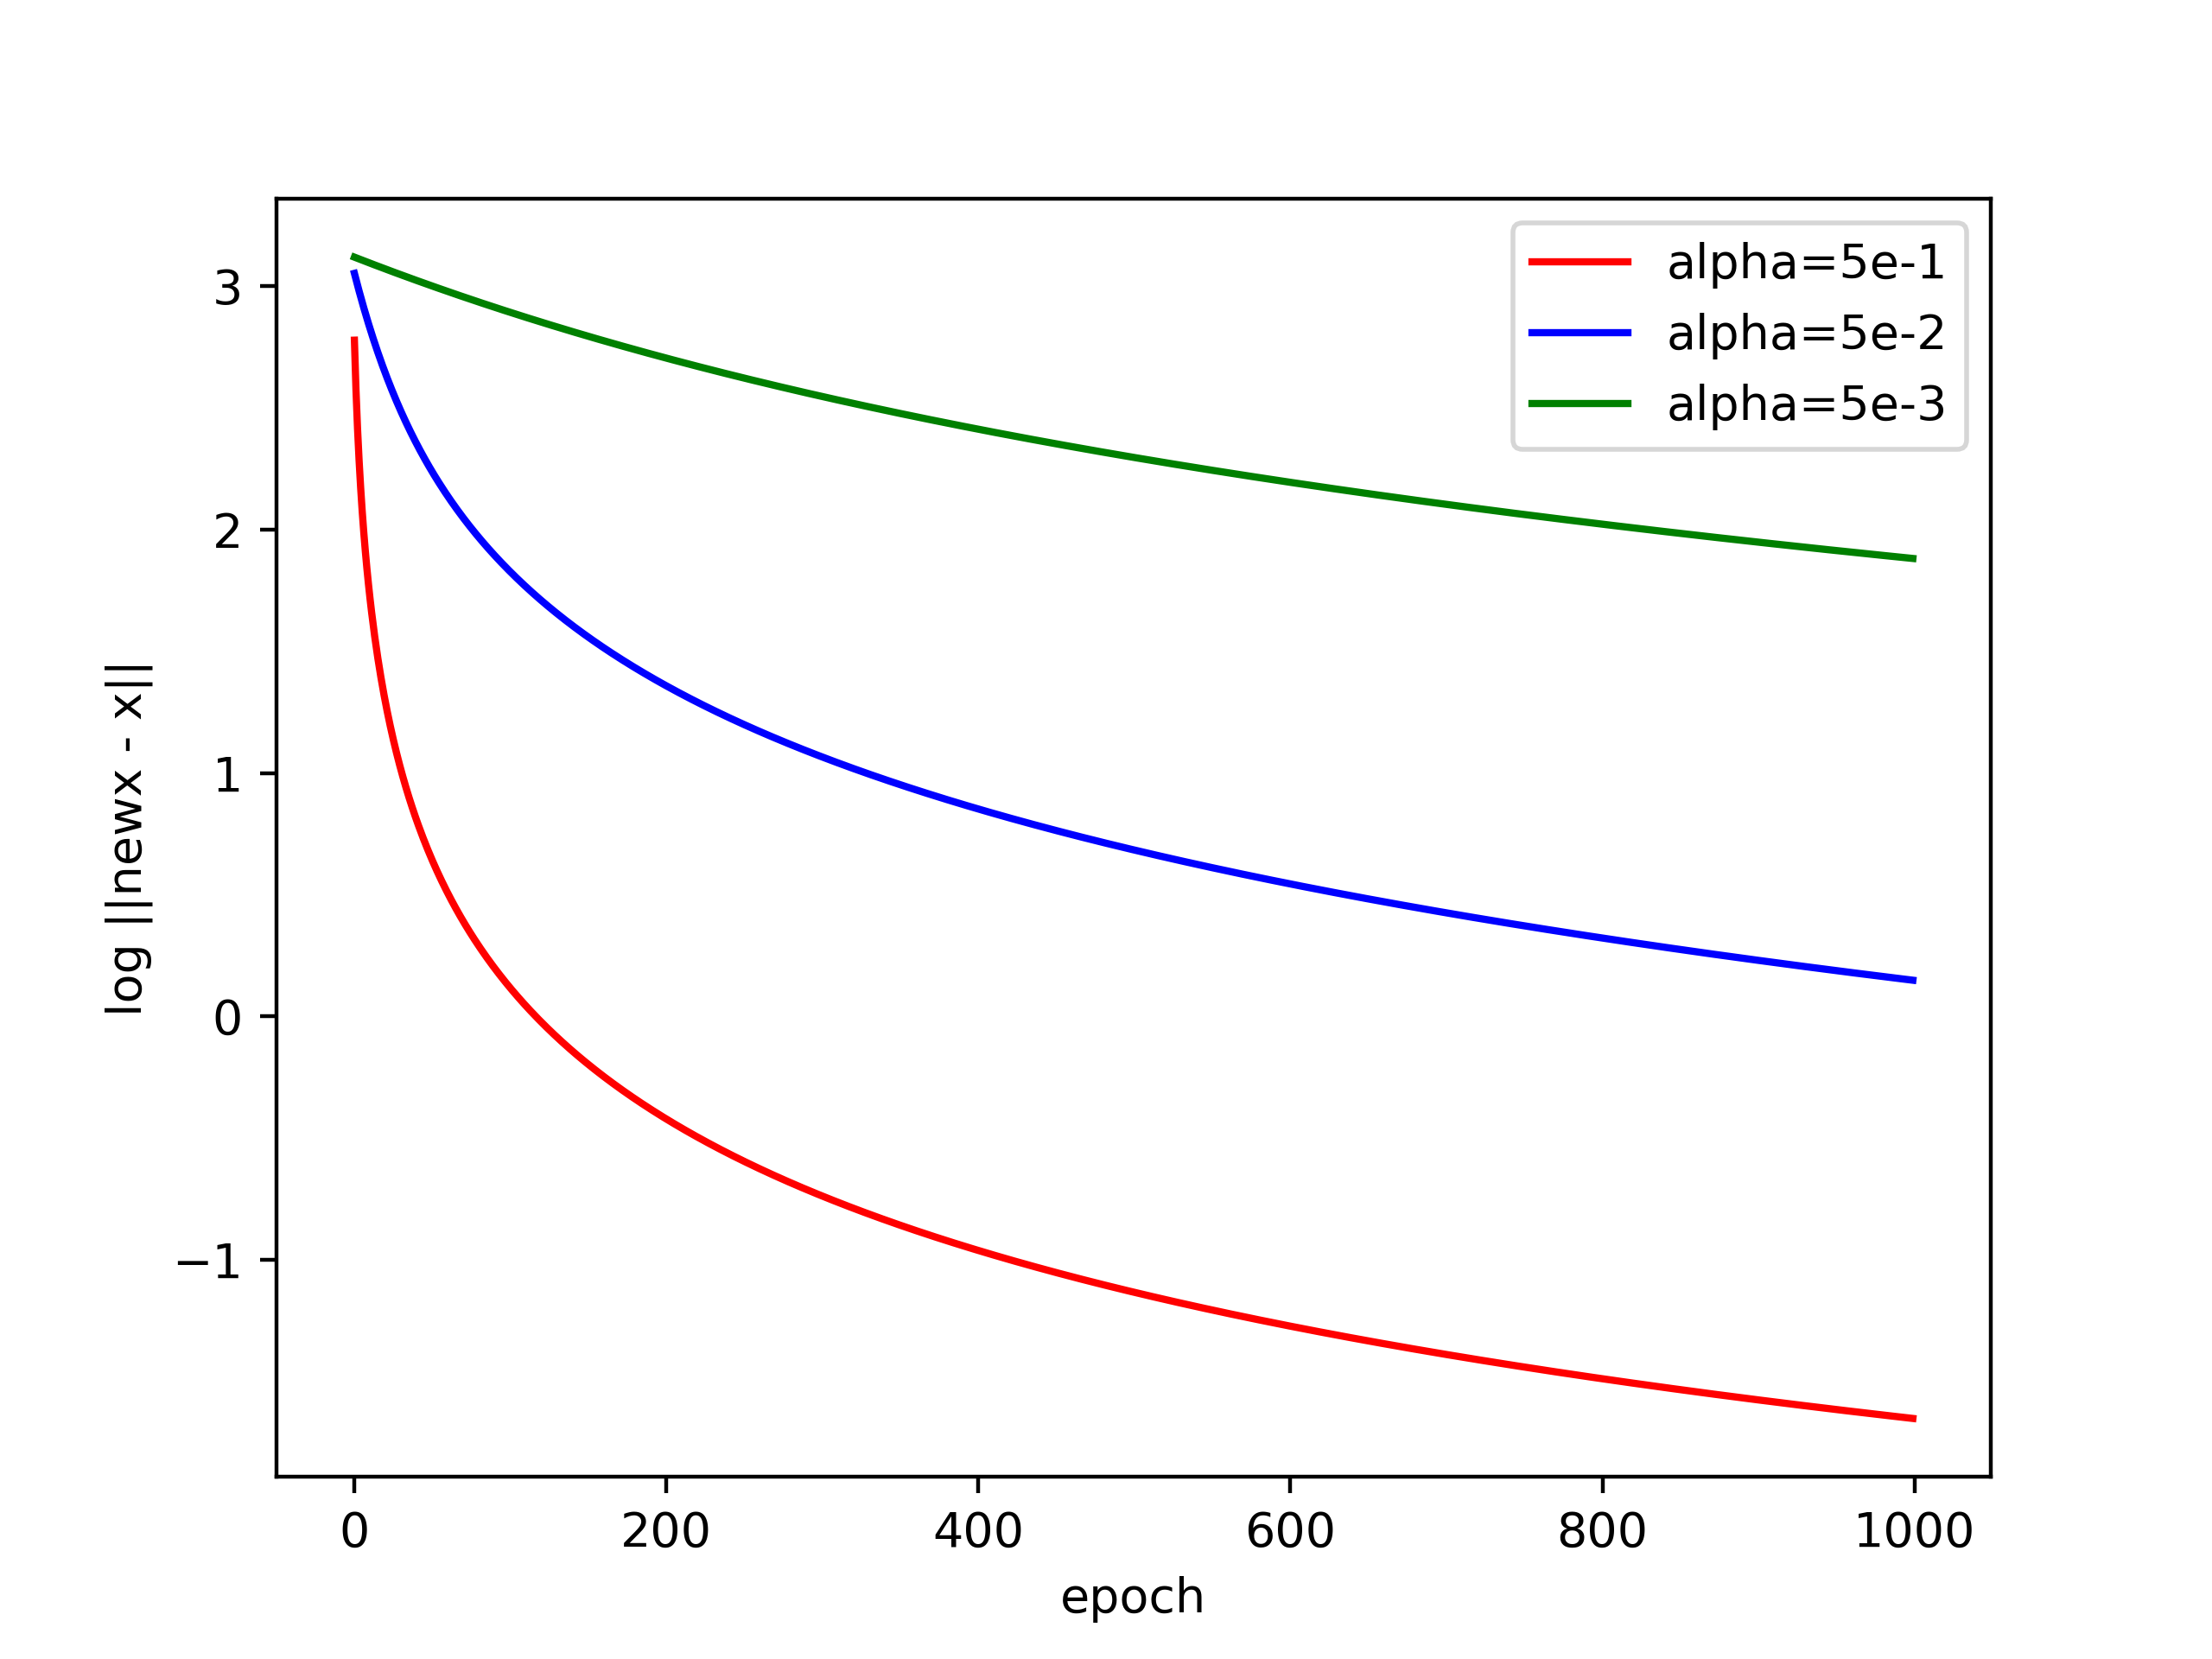
\includegraphics[width=150mm]{./Figures/gd-log.png}
        \caption{Python实现梯度下降法求解最小二乘问题}
        \label{figure_gd}
    \end{figure}
\end{solution}
